% Options for packages loaded elsewhere
\PassOptionsToPackage{unicode}{hyperref}
\PassOptionsToPackage{hyphens}{url}
%
\documentclass[
]{report}
\usepackage{amsmath,amssymb}
\usepackage[letterpaper, margin=2.5cm]{geometry} % Perfect margins
\usepackage{setspace} % Spacing
\onehalfspacing % Elegant line spacing
\usepackage{fancyhdr} % Premium header/footer
\usepackage{titlesec} % Beautiful section headers

% Configuración de Encabezado y Pie de página profesional
\pagestyle{fancy}
\fancyhf{}
\fancyhead[L]{\small\itshape Universidad Peruana Unión}
\fancyhead[R]{\small\itshape Perfil de Proyecto}
\fancyfoot[C]{\thepage}
\renewcommand{\headrulewidth}{0.4pt}
\setlength{\headheight}{15pt}

% Configuración visual de secciones académicas
\titleformat{\section}{\large\bfseries\color{blue!70!black}}{\thesection}{1em}{}
\titleformat{\subsection}{\normalsize\bfseries\color{black!90!white}}{\thesubsection}{1em}{}

\usepackage{newtxtext,newtxmath} % Times Roman style typography
\usepackage{iftex}
\ifPDFTeX
  \usepackage[T1]{fontenc}
  \usepackage[utf8]{inputenc}
  \usepackage{textcomp} % provide euro and other symbols
\else % if luatex or xetex
  \usepackage{unicode-math}
  \defaultfontfeatures{Scale=MatchLowercase}
  \defaultfontfeatures[\rmfamily]{Ligatures=TeX,Scale=1}
\fi
% Use upquote if available, for straight quotes in verbatim environments
\IfFileExists{upquote.sty}{\usepackage{upquote}}{}
\IfFileExists{microtype.sty}{% use microtype if available
  \usepackage[]{microtype}
  \UseMicrotypeSet[protrusion]{basicmath} % disable protrusion for tt fonts
}{}
\makeatletter
\@ifundefined{KOMAClassName}{% if non-KOMA class
  \IfFileExists{parskip.sty}{%
    \usepackage{parskip}
  }{% else
    \setlength{\parindent}{0pt}
    \setlength{\parskip}{6pt plus 2pt minus 1pt}}
}{% if KOMA class
  \KOMAoptions{parskip=half}}
\makeatother
\usepackage{xcolor}
\IfFileExists{xurl.sty}{\usepackage{xurl}}{} % add URL line breaks if available
\IfFileExists{bookmark.sty}{\usepackage{bookmark}}{\usepackage{hyperref}}
\hypersetup{
  hidelinks,
  pdfcreator={LaTeX via pandoc}}
\urlstyle{same} % disable monospaced font for URLs
\usepackage{longtable,booktabs,array}
\usepackage{calc} % for calculating minipage widths
% Correct order of tables after \paragraph or \subparagraph
\usepackage{etoolbox}
\makeatletter
\patchcmd\longtable{\par}{\if@noskipsec\mbox{}\fi\par}{}{}
\makeatother
% Allow footnotes in longtable head/foot
\IfFileExists{footnotehyper.sty}{\usepackage{footnotehyper}}{\usepackage{footnote}}
\makesavenoteenv{longtable}
\usepackage{graphicx}
\makeatletter
\def\maxwidth{\ifdim\Gin@nat@width>\linewidth\linewidth\else\Gin@nat@width\fi}
\def\maxheight{\ifdim\Gin@nat@height>\textheight\textheight\else\Gin@nat@height\fi}
\makeatother
% Scale images if necessary, so that they will not overflow the page
% margins by default, and it is still possible to overwrite the defaults
% using explicit options in \includegraphics[width, height, ...]{}
\setkeys{Gin}{width=\maxwidth,height=\maxheight,keepaspectratio}
% Set default figure placement to htbp
\makeatletter
\def\fps@figure{htbp}
\makeatother
\setlength{\emergencystretch}{3em} % prevent overfull lines
\providecommand{\tightlist}{%
  \setlength{\itemsep}{0pt}\setlength{\parskip}{0pt}}
\setcounter{secnumdepth}{-\maxdimen} % remove section numbering
\ifLuaTeX
  \usepackage{selnolig}  % disable illegal ligatures
\fi

\author{}
\date{}

\begin{document}

\begin{titlepage}
\thispagestyle{empty}
\begin{center}
    \large\textbf{UNIVERSIDAD PERUANA UNIÓN} \\
    \vspace{0.2cm}
    \large FACULTAD DE INGENIERÍA Y ARQUITECTURA \\
    \vspace{0.1cm}
    \normalsize Escuela Profesional de Ingeniería de Sistemas \\
    
    \vspace{1.0cm}
    
\includegraphics[width=3.71528in,height=2.08984in]{./media/image1.png} \\
    \vspace{1.0cm}
    
    \large\textbf{Perfil de proyecto de investigación} \\
    \vspace{0.8cm}
    
    \large\textbf{"Sistema de Predicción Geográfica de Desnutrición Crónica Infantil en el Perú mediante un Modelo Híbrido de Machine Learning"} \\
    
    \vspace{1.2cm}
    \normalsize
    Por: \\
    \vspace{0.2cm}
    Abel Is-Boset Guevara Huasco (0009-0001-4809-6430) \\
    Zulin Pamela Vallejos Cotrina (0009-0004-1485-2981) \\
    Verónica Lisseth Vergara Rojas (0009-0007-3256-9823) \\
    
    \vspace{0.8cm}
    Asesor: \\
    \vspace{0.1cm}
    Asesor (Grado académico. Nombres y Apellidos, Arial 14, sin negrita) \\
    
    \vspace{0.6cm}
    Linea de investigación: \\
    
    \vfill
    \textbf{Lima, noviembre de 2025}
\end{center}
\end{titlepage}
\newpage

\section{1. Planteamiento del Problema}\label{planteamiento-del-problema}

\subsection{1.1 Identificación del problema}\label{identificaciuxf3n-del-problema}

La desnutrición crónica infantil constituye uno de los principales desafíos de salud pública a nivel mundial, afectando el desarrollo físico, cognitivo y social de millones de niños menores de cinco años. Según la Organización Mundial de la Salud (OMS) y UNICEF, más del 22 \% de los niños en países en desarrollo presenta retraso en el crecimiento, una condición estrechamente vinculada con la pobreza, la inseguridad alimentaria y las desigualdades territoriales {[}1, 2{]}. Este problema no solo compromete el bienestar y la calidad de vida de la infancia, sino que también limita el progreso económico y social de las naciones, dificultando el cumplimiento del Objetivo de Desarrollo Sostenible 2: Hambre Cero {[}3{]}.

La desnutrición infantil es un fenómeno complejo influido por múltiples
factores interrelacionados como las condiciones económicas, la educación
materna, el acceso a servicios básicos, la calidad del entorno ambiental
y las desigualdades territoriales {[}4, 5{]}. Estas variables no
actúan de forma aislada, sino que se combinan generando distintos
niveles de vulnerabilidad según el espacio geográfico. Comprender cómo
se distribuye y evoluciona la desnutrición en el territorio resulta
esencial para diseñar estrategias de intervención más precisas. En este
contexto, los modelos inteligentes han permitido avances significativos
en el análisis y pronóstico del estado nutricional, mediante el uso de
algoritmos de clasificación y regresión que estiman tendencias y
factores de riesgo {[}6{]}. Sin embargo, estos enfoques tradicionales
aún presentan limitaciones, ya que suelen basarse en un número
restringido de variables y no logran capturar la interacción entre
componentes sociales, ambientales y territoriales {[}7{]}. Por ello, se
plantea la necesidad de explorar modelos más robustos y adaptativos que
incorporen nuevas variables con características heterogéneas, capaces de
aportar mayor precisión a las predicciones y reflejar de manera más
realista la complejidad del fenómeno.

Diversas investigaciones recientes han empleado métodos estadísticos y
de machine learning para analizar la desnutrición infantil, logrando
avances significativos en la clasificación del estado nutricional y la
identificación de factores asociados. Modelos híbridos y de ensamble,
como los propuestos por Alam et al. (2025) y Hadikurniawati et al.
(2025), alcanzaron altos niveles de precisión al integrar variables
antropométricas, demográficas y socioeconómicas {[}8, 9{]}.
Asimismo, estudios con enfoque espacial como los de Habtewold et al.
(2025) y Egbon et al. (2022) incorporaron análisis bayesianos y
geográficos para identificar zonas críticas y patrones territoriales del
riesgo nutricional {[}10, 11{]}. Estas experiencias evidencian el
potencial de la inteligencia artificial para mejorar el diagnóstico y
pronóstico de la desnutrición infantil, especialmente en contextos donde
la información es limitada o dispersa.

A pesar de estos avances, se identifican limitaciones metodológicas
específicas que restringen la aplicabilidad y generalización de los
modelos existentes. En primer lugar, muchos estudios se han desarrollado
en contextos internacionales y se centran en variables individuales, sin
integrar adecuadamente las dimensiones ambientales, sanitarias o
territoriales. Además, el tratamiento de los datos espaciales y
socioeconómicos presenta dificultades por la diferencia en sus escalas,
unidades y niveles de precisión {[}12{]}. Varios autores reconocen que
el desempeño predictivo se ve afectado por la heterogeneidad de las
fuentes, la falta de estandarización de los indicadores y la ausencia de
técnicas capaces de vincular de manera coherente los datos tabulares con
la información geográfica {[}11, 13{]}. Estas limitaciones reducen
la capacidad de los modelos para representar la realidad territorial del
problema y detectar zonas de alta vulnerabilidad nutricional con
suficiente precisión {[}14{]}

Frente a este telón de fondo, la gran prueba que se nota se encuentra en
cómo se manejan y juntan cosas distintas, cada una con sus propios
tamaños, formas y cuán detallada es. Esas distintas maneras piden usar
trucos concretos para cambiarlas, hacerlas parejas y estudiarlas, lo que
hace más difícil armar el modelo y que las fuentes se entiendan bien.
Este problema de método sugiere que hacen falta caminos más listos que
unan diferentes maneras de tratar y aprender de máquinas, dejando que se
vea cómo se influyen las piezas y haciendo que las cuentas que hacen los
modelos sean mejores en situaciones verdaderas y complicadas.

En el caso del Perú, la desnutrición crónica infantil continúa siendo un
problema estructural a pesar de los avances logrados. Según la Encuesta
Demográfica y de Salud Familiar (ENDES, 2023), la prevalencia nacional
alcanza el 11,5 \%, con regiones como Huancavelica y Loreto que superan
el 20 \% {[}15{]}. Esta desigualdad refleja que el problema responde
también a factores socioeconómicos, sanitarios y ambientales. Sin
embargo, los estudios nacionales aún no aplican enfoques predictivos ni
análisis geoespaciales que permitan anticipar zonas de riesgo {[}16{]}.
Por lo tanto, se evidencia la necesidad de impulsar modelos híbridos de
machine learning y análisis geoespacial que integren múltiples tipos de
variables, permitiendo un análisis más completo, objetivo y preciso de
la desnutrición crónica infantil en el país.

\hypertarget{justificaciuxf3n}{%
\subsection{1.2 Justificación}\label{justificaciuxf3n}}

Desde el ámbito teórico, este estudio contribuye al conocimiento
existente al incorporar los determinantes sociales, ambientales y
espaciales en el análisis de la desnutrición infantil mediante enfoques
de machine learning {[}17{]}. Esta integración permite comprender con
mayor profundidad las interacciones no lineales entre factores
demográficos, geográficos y de infraestructura básica, superando las
limitaciones de los modelos estadísticos tradicionales centrados
únicamente en variables antropométricas {[}15{]}. Asimismo, aporta
evidencia científica sobre el potencial de la inteligencia artificial
para abordar problemas de salud pública desde una perspectiva
multidimensional, fortaleciendo el marco conceptual para futuras
investigaciones relacionadas con el análisis predictivo del estado
nutricional infantil {[}18{]}.

Desde el punto de vista práctico, la propuesta busca desarrollar un
sistema de pronóstico geoespacial que permita identificar zonas con
mayor probabilidad de desnutrición crónica infantil y estimar escenarios
de riesgo nutricional a nivel local o regional. El modelo procesará
información proveniente de fuentes oficiales como censos, encuestas
demográficas y registros ambientales para generar mapas predictivos,
reportes y visualizaciones dinámicas que faciliten la interpretación de
resultados. De esta manera, las instituciones públicas como el
Ministerio de Salud, el MIDIS y los gobiernos regionales, así como
organismos de cooperación o centros de investigación, podrán utilizar
los resultados para priorizar intervenciones preventivas, optimizar la
distribución de recursos y mejorar la focalización de programas sociales
{[}16{]}. Además, el proyecto fortalecerá las competencias del equipo
investigador en el uso de tecnologías de analítica de datos aplicadas al
ámbito social y territorial {[}19, 20{]}

Desde el enfoque innovador, el estudio propone la integración de modelos
híbridos de machine learning con análisis geoespacial, un enfoque poco
explorado en el contexto peruano. Esta combinación permite no solo
incrementar la precisión de las predicciones, sino también representar
la dimensión territorial de la desnutrición infantil con mayor
realismo {[}21{]}. El carácter híbrido del modelo, al incorporar
diferentes técnicas de procesamiento y aprendizaje, amplía las
posibilidades de investigación en ingeniería aplicada a la salud y
ofrece un marco metodológico replicable para abordar otras problemáticas
sociales mediante la inteligencia artificial y la ciencia de datos
{[}22{]}

\hypertarget{estado-del-arte}{%
\subsection{1.3 Estado del Arte}\label{estado-del-arte}}

Durante la última década, el avance de la inteligencia artificial (IA) y
del análisis geoespacial ha permitido transformar el estudio de la
desnutrición infantil, pasando de enfoques descriptivos a modelos
predictivos capaces de anticipar escenarios de riesgo nutricional con
alta precisión. Estas herramientas combinan información sanitaria,
socioeconómica, ambiental y geográfica, generando una visión más
integral del problema y posibilitando la planificación temprana de
estrategias preventivas {[}23, 24{]}. En regiones de baja
disponibilidad de datos, los enfoques de modelado espacial y aprendizaje
automático han demostrado ser una alternativa efectiva para mejorar la
estimación de indicadores nutricionales {[}25{]}.

En África Subsahariana, Backer y Billing {[}26{]} desarrollaron un
modelo basado en Random Forest para predecir la prevalencia de
desnutrición aguda infantil considerando variables ambientales y de
conflicto en 36 países. El modelo logró pronósticos a 12 meses con alta
capacidad predictiva, demostrando la relevancia de los factores
climáticos y de inestabilidad como predictores nutricionales. En la
misma región, Tadesse {[}27{]} aplicó un enfoque de Gradient Boosting
para pronosticar desnutrición infantil en Kenia utilizando datos del
sistema DHIS2 combinados con señales satelitales (MODIS-GPP), alcanzando
un AUC de 0.86 en predicciones a seis meses. Resultados similares se
observaron en estudios sobre determinantes nutricionales realizados en
Asia del Sur, donde Rahut et al. {[}23{]} identificaron la interacción
entre variables climáticas, de pobreza y acceso a servicios básicos como
principales predictores de desnutrición crónica infantil.

En el ámbito del análisis espacial, Aheto {[}28{]} propuso un modelo
bayesiano espaciotemporal para estimar la desnutrición crónica en Ghana,
generando mapas predictivos de riesgo nutricional y destacando la
influencia del nivel educativo materno sobre el crecimiento infantil. De
forma complementaria, Jasper et al. {[}18{]} aplicaron modelos
geostatísticos bayesianos para mapear la desnutrición aguda severa en
Papúa (Indonesia), alcanzando una resolución de 1 × 1 km y demostrando
la utilidad del mapeo de alta frecuencia en zonas con escasa información
censal. Mgomezulu et al. {[}13{]} extendieron este enfoque mediante
modelos híbridos y de aprendizaje profundo en Malawi, combinando
algoritmos de ensamble (Random Forest, XGBoost) con técnicas de balanceo
de clases (SMOTE) sobre datos del Living Standards Measurement Survey,
logrando una precisión del 99 \%. Estos hallazgos refuerzan la necesidad
de integrar componentes espaciales y sociales en los modelos de
predicción nutricional.

Por su parte, Hadikurniawati et al. {[}29{]} diseñaron un modelo híbrido
de doble fusión con atención (Dual-Fusion Hybrid Model), que combina
redes neuronales convolucionales 1D con clasificadores tradicionales
para procesar variables antropométricas y demográficas. Su arquitectura
obtuvo una exactitud del 99.7 \%, confirmando que la fusión de métodos
supervisados y no supervisados mejora la capacidad de generalización y
reduce sesgos en conjuntos de datos complejos y desbalanceados. De modo
similar, Santoso et al {[}30{]} desarrollaron un modelo de IA explicable
con atención múltiple, integrando redes CNN-LSTM-MHA para clasificar
estados nutricionales con mayor transparencia e interpretabilidad. Ambos
enfoques evidencian la transición hacia sistemas predictivos
inteligentes que combinan rendimiento técnico y capacidad explicativa.

En el contexto del modelado predictivo, estudios recientes han
incorporado la dimensión temporal para anticipar fluctuaciones en la
malnutrición aguda. Constenla-Villoslada et al. {[}31{]} demostraron que
el monitoreo de alta frecuencia junto con modelos de machine learning
permite pronosticar brotes de desnutrición aguda en Kenia con semanas de
anticipación, combinando datos climáticos, de precios de alimentos y de
mercado. De igual manera, Egbon et al. {[}11{]} aplicaron un enfoque
bayesiano bivariado espacial para estimar la concurrencia entre
desnutrición crónica y aguda en Etiopía, destacando la correlación
espacial entre ambos indicadores. Alam et al. {[}18{]} propusieron un
marco de inteligencia artificial híbrida para clasificar el estado
nutricional en 74 países, validando la eficacia de los modelos
evolutivos en contextos multiculturales.

Juntos, estos trabajos muestran más fuerza del aprendizaje de máquinas.
También, la unión de datos de muchas áreas ayuda a ver la desnutrición
infantil antes de que pase. Pero, casi toda la ciencia se fija en Asia o
África. Estos estudios ven solo medidas del cuerpo de cada niño. No
juntan a la vez las causas sociales, del medio ambiente y del lugar.
Además, los modelos nuevos que mezclan cosas y ven el espacio funcionan
muy bien. Sin embargo, se usan poco en América Latina. Allí, las formas
del mapa y las faltas de igualdad piden nuevos modos de hacer las cosas.
Por esto, crear modelos predictivos mixtos con mapas para Perú es un
paso lógico. Esto sigue la idea actual de la ciencia. Ayudará a mejorar
el cuidado y las decisiones de salud. Usa para esto la inteligencia
artificial y la información de mapas {[}32{]}

\subsection{1.4 Objetivos}\label{objetivos}

\subsubsection*{Objetivo General}

Desarrollar un Sistema de Predicción Geográfica de Desnutrición Crónica Infantil en el Perú mediante un Modelo Híbrido de Machine Learning, que permita identificar y visualizar territorialmente las zonas de mayor riesgo nutricional, mejorando la precisión y capacidad predictiva del análisis.

\subsubsection*{Objetivos Específicos}

\begin{itemize}
\item
  \textbf{Analizar y establecer} las variables determinantes asociadas a
  la desnutrición crónica infantil en el Perú, utilizando microdatos de
  fuentes oficiales agregados por zona geográfica.
\item
  \textbf{Depurar y estructurar} el corpus de datos sobre el estado
  nutricional infantil por distrito y departamento, integrando las
  variables relevantes en series temporales zonales para su utilización
  en el modelado predictivo.
\item
  \textbf{Implementar un Modelo Híbrido de Machine Learning} que integre
  variables demográficas, sanitarias y ambientales por zona, para
  generar mapas predictivos de riesgo de desnutrición crónica infantil a
  nivel distrital y departamental en el Perú.
\item
  \textbf{Evaluar} la precisión, desempeño y capacidad explicativa del
  modelo propuesto a partir de métricas de validación internas,
  determinando su nivel de eficacia en la predicción geográfica de la
  desnutrición crónica infantil.
\end{itemize}

\hypertarget{hipuxf3tesis}{%
\subsection{1.5 Hipótesis}\label{hipuxf3tesis}}

\begin{itemize}
\item
  La aplicación de modelos híbridos de \emph{machine learning} optimiza
  la exactitud y el desempeño predictivo en la identificación
  geoespacial de zonas con alto riesgo de desnutrición crónica infantil,
  proporcionando resultados más consistentes para el análisis
  territorial.
\item
  La precisión y capacidad explicativa del modelo predictivo se verán
  incrementadas al integrar nuevas variables en el corpus de datos,
  permitiendo una estimación más completa y fiable del riesgo de
  desnutrición crónica infantil.
\end{itemize}

\hypertarget{variables}{%
\subsection{1.6 Variables}\label{variables}}

Variable independiente: \textbf{Sistema de Predicción Geográfica basado
en modelos híbridos de Machine Learning}

Representa una herramienta tecnológica inteligente que integra datos
espaciales, socioeconómicos y ambientales con algoritmos predictivos de
inteligencia artificial, con el propósito de anticipar escenarios de
riesgo nutricional infantil y generar mapas de alerta temprana útiles
para la gestión preventiva en salud pública. Este tipo de enfoque
híbrido combina la capacidad analítica del \emph{machine learning} con
la contextualización geoespacial, permitiendo mejorar la precisión y
oportunidad del pronóstico nutricional

Variable dependiente: \textbf{Desnutrición Crónica Infantil}

El retraso en el crecimiento físico se llama desnutrición crónica infantil. Afecta el desarrollo mental de niños de menos de cinco años. Esto pasa por no comer suficientes nutrientes por mucho tiempo. También influyen malos servicios de salud y problemas del lugar donde viven. Los factores económicos dificultan su buen desarrollo. La Organización Mundial de la Salud dice cómo se mide. Miden la altura de los niños para su edad. Debe ser muy baja comparada con el estándar de la OMS {[}1, 10{]}.

En nuestra investigación, esta medida es el resultado principal del sistema que predice. Sin embargo, miramos esto de forma más amplia. Agregamos nuevas cosas importantes. Incluimos datos del lugar y el ambiente. Vemos el clima y qué tan vulnerable es la zona. También vemos si tienen acceso a servicios. Hacemos esto para predecir mejor. Queremos entender todas las causas de la desnutrición en Perú.

\hypertarget{metodologuxeda}{%
\section{2. Metodología}\label{metodologuxeda}}

\hypertarget{diseuxf1o-metodoluxf3gico}{%
\subsection{2.1 Diseño Metodológico}\label{diseuxf1o-metodoluxf3gico}}

Este estudio se hará usando el método CRISP-DM. Este es el sistema que
se usa más a nivel mundial. Sigue el proceso para la minería de datos.
Es el estándar para todo proyecto de datos. También funciona para la
inteligencia artificial {[}33{]}. Este plan da una forma clara. Funciona
en pasos que se pueden repetir. Se puede revisar todo el trabajo. Este
sistema ayuda a manejar todas las partes. Cubre ver el tema hasta poner
el programa final. Asegura que el resultado se pueda seguir. Muestra lo
que se hizo. Da valor técnico al trabajo hecho.

El enfoque de la investigación es cuantitativo, aplicado, descriptivo y
predictivo, orientado al diseño, entrenamiento y validación de un
sistema de pronóstico geoespacial de la desnutrición crónica infantil en
el Perú, utilizando técnicas de inteligencia artificial híbrida y
modelos bayesianos espaciales. El estudio es de tipo no experimental,
dado que no se manipulan variables independientes y los datos serán
analizados tal como fueron recolectados por las instituciones oficiales.
Asimismo, el diseño es longitudinal de tendencia, porque se emplean
bases de datos secundarias correspondientes a los últimos cinco años
(ENDES 2019--2024) con el propósito de evaluar cómo cambia una variable
en la población a lo largo del tiempo, sin seguir a las mismas personas.

De acuerdo con Wirth y Hipp {[}33{]}el modelo CRISP-DM estructura un
proyecto de minería de datos en seis fases iterativas: comprensión del
negocio, comprensión de los datos, preparación de los datos, modelado,
evaluación y despliegue. Estas fases se adaptan en el presente trabajo
al desarrollo del producto de ingeniería, conformando un proceso
sistemático que combina los componentes analíticos, computacionales y
geoespaciales del sistema propuesto.

\begin{center}
    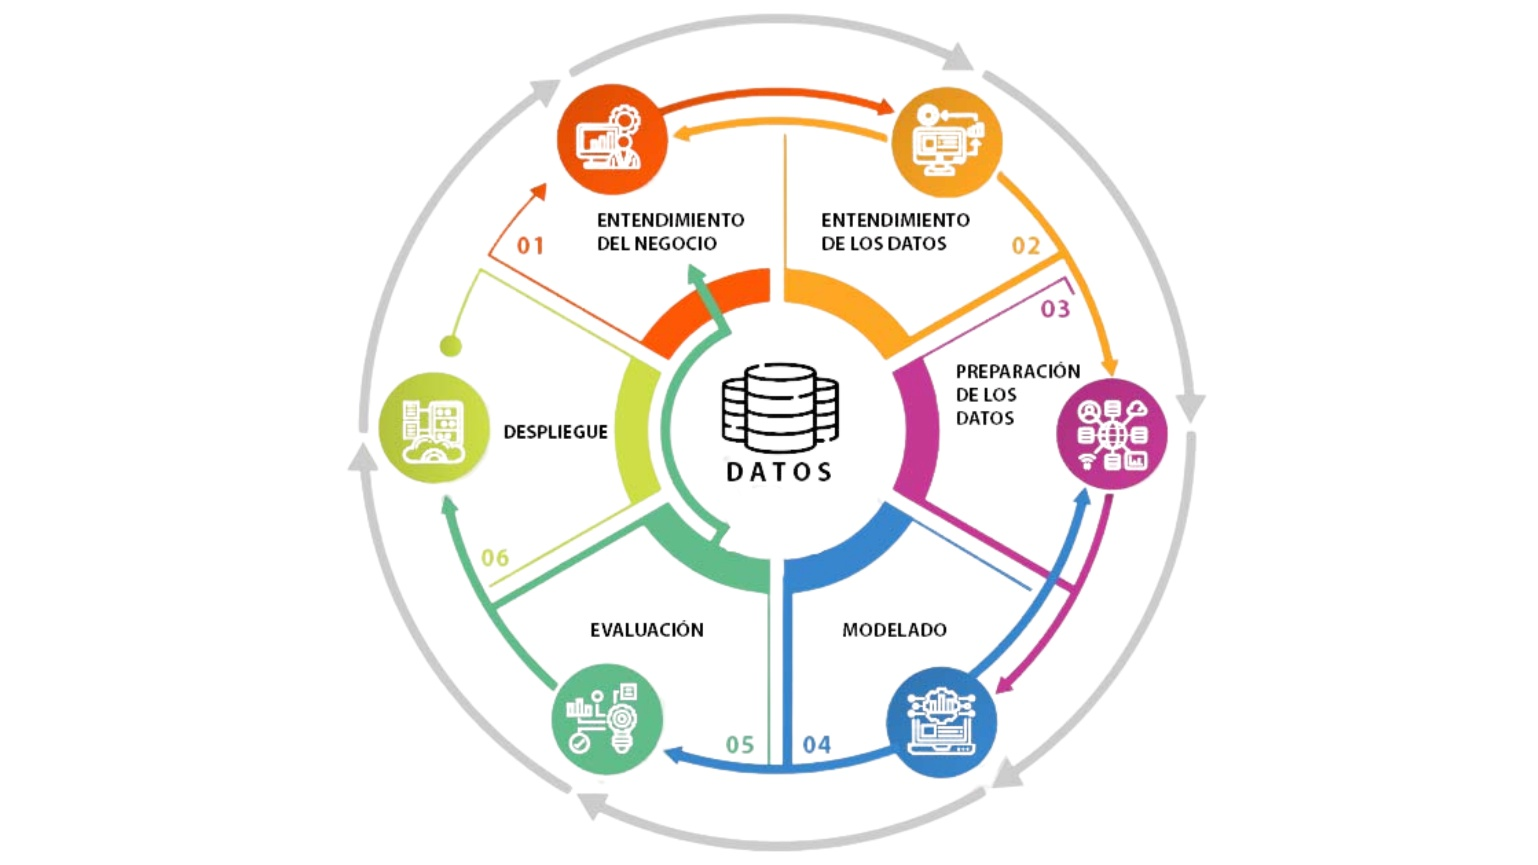
\includegraphics[width=4.46187in,height=3.92361in]{./media/image2.jpeg}
    
    \small Fig. 1. Fases del modelo metodológico CRISP-DM y su naturaleza iterativa. Adaptado de Wirth y Hipp.
\end{center}

\textbf{Procedimiento para la construcción del producto de ingeniería
según CRISP-DM}

A continuación, se describe el procedimiento seguido para la
construcción del producto de ingeniería según las fases del modelo
CRISP-DM.

\textbf{Fase I: Comprensión del negocio}

En esta etapa inicial, vamos a estudiar el problema. Es la falta de
nutrición en niños peruanos. Buscaremos las causas. Estas causas son
sociales, de la gente y del lugar. Veremos qué influye en que esto pase
tanto. Se hará una revisión de estudios previos. Estos son del país y de
otros lados. Esto servirá para entender el tema. También se fijarán las
metas claras del programa. De este estudio, saldrán las cuentas
importantes. El modelo debe predecir esas cuentas. Se verán también las
necesidades del equipo. Además, se trazará el primer diseño del sistema.
Este diseño mostrará las partes de análisis. Mostrará cómo se moverá la
información. También se detallarán los bloques del sistema. Esta fase
permitirá transformar el problema social en un problema de ingeniería de
datos, articulando las necesidades de información con las capacidades
predictivas del sistema.

\textbf{Fase II: Comprensión de los datos}

En esta etapa, se revisarán los datos pequeños de ENDES. Usaremos los
datos del INEI que cubren los años 2019 a 2024. Estos archivos tienen
datos de salud y hogar. También incluyen información de comida y
nutrición. Se mirará la forma de los archivos. Veremos qué datos hay.
También se revisará si los datos son buenos. Hay que juzgar qué tan
completos son los datos de nutrición infantil. Esto incluye la edad y el
sexo. Se verá la altura y la edad de la madre. También se verá la zona
donde viven. Haremos informes con números y gráficos. Esto ayuda a ver
cómo se reparten los datos. Así se hallan errores. Entender esto sirve
para elegir datos claves. También sirve para fijar cómo dividir grupos
para los siguientes estudios. Constenla-Villoslada y otros {[}31{]}
dicen que usar datos de tiempo y de gente mejora las predicciones de
nutrición.

\textbf{Fase III: Preparación de los datos}

En este punto haremos que los datos estén listos para el diseño del
modelo. Se arreglarán las notas que estén a medias, se rellenarán los
huecos con números usando trucos de números y se nivelarán las cifras
para que todo esté a la misma altura. También, se pondrán códigos a las
cosas de grupo y se usarán trucos para achicar el espacio, como la Piel
de Componentes Fundamentales (la variación PCA del núcleo), para que el
diseño corra mejor {[}34{]}.

Aparte, se pondrá el método SMOTE (Técnica de Sobremuestra Sintética de
Minorías) {[}35{]} para equilibrar cómo se reparten los tipos y que el
ensayo del patrón no se incline hacia un lado, usando la Escala Mínima
Máxima. Alam {[}18{]} piensa que si los datos están bien arreglados,
esto ayuda mucho a que los diseños mixtos de mente artificial sean más
exactos y firmes. Esta parte asegurará que la información sea pareja,
que muestre lo que debe y que sirva para las maneras de aprender que
usaremos.

\textbf{Fase IV: Modelado}

En esta etapa se levantará la estructura mixta de predicción, juntando
métodos de saber profundo enfocados en información ordenada con un trozo
de espacio. Se usará una red neuronal apretada (DNN) para manejar las
medidas del cuerpo, edad y cosas de la madre, mientras que las zonas
geográficas se codificarán con representaciones espaciales, dejando ver
vínculos espaciales ocultos mejor que las maneras de etiqueta viejas.
También, si existe una tabla de cercanía de territorios, se añadirá una
Red Neuronal de Grafos (GNN) extra para dibujar la dependencia mutua de
lugar entre zonas y áreas {[}10, 31{]}.\\
La práctica de enseñanza se llevará a cabo usando los datos ENDES de los
tiempos 2019 a 2023, guardando los del tiempo 2024 para chequear el
aparato. De acuerdo con escritos, juntar representaciones espaciales y
redes apretadas sube la eficacia y acierto en sitios con mucha mezcla de
espacio y grupos de personas {[}36{]}. Esta parte dejará crear un
aparato mezclado con aptitud para juntar figuras.

\begin{center}
    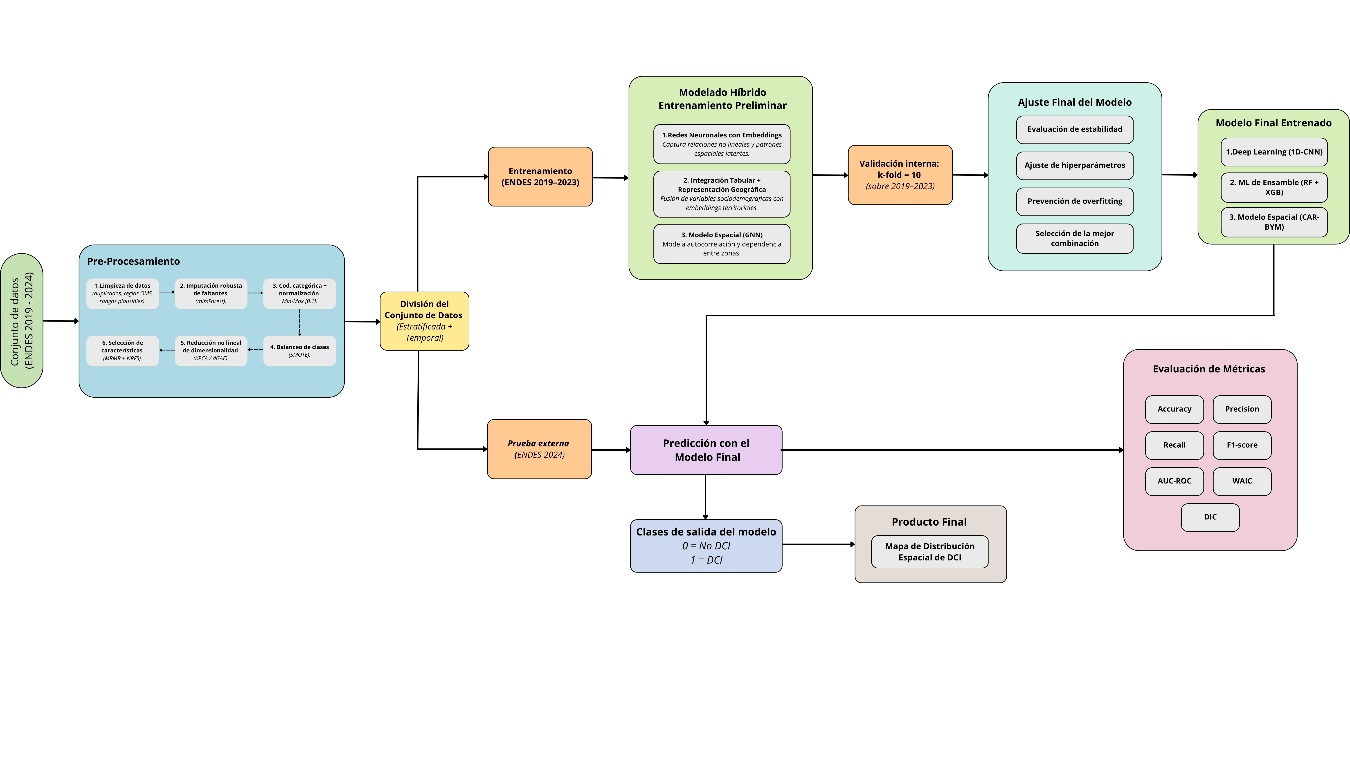
\includegraphics[width=0.9\linewidth]{./media/image3.jpeg}
    
    \small Fig. 2. Arquitectura del modelado híbrido propuesto.
\end{center}

\textbf{Fase V: Evaluación}

En esta fase se evaluará el desempeño del modelo híbrido de pronóstico
utilizando un enfoque mixto de validación, que combina una validación
cruzada interna k-fold (k = 10) con una evaluación externa
independiente.

Los datos correspondientes a los años 2019--2023 se emplearán para el
entrenamiento y ajuste de los modelos, aplicando la validación cruzada
k-fold con el propósito de estimar la variabilidad del rendimiento y
seleccionar los hiperparámetros óptimos.

Posteriormente, los datos del año 2024 se reservarán como conjunto de
prueba externo, el cual se utilizará una sola vez para medir la
capacidad de generalización y estabilidad temporal del sistema.

Se aplicarán métricas de desempeño tales como Accuracy, Precision,
Recall, F1-score, AUC, WAIC y DIC, que permitirán analizar tanto la
calidad de las predicciones como el nivel de ajuste alcanzado por el
sistema en sus componentes predictivos y espaciales {[}37{]}.

Dado que la arquitectura integra diferentes técnicas en un mismo flujo
de procesamiento, la evaluación se centrará en el rendimiento global del
modelo híbrido, considerando la precisión predictiva del módulo de
\emph{ensemble learning} y la coherencia espacial del componente
bayesiano (CAR-BYM).

\textbf{Fase VI: Despliegue}

Finalmente, se procederá al despliegue del modelo en un entorno de
visualización interactivo desarrollado con Power BI o Streamlit. El
sistema integrará módulos para la carga de datos, ejecución del modelo y
visualización de resultados. La interfaz permitirá explorar los
indicadores nutricionales, visualizar los mapas de riesgo y analizar las
tendencias anuales por departamento y distrito.

\hypertarget{diseuxf1o-muestral}{%
\subsection{2.2 Diseño muestral}\label{diseuxf1o-muestral}}

\textbf{Población y Muestra}

La unidad de análisis estará constituida por cada registro individual
proveniente de la ENDES, correspondiente a un menor incluido en el
módulo de nutrición durante el periodo 2019--2024. Cada observación
contiene información antropométrica, sanitaria y sociodemográfica
relevante. Este grupo es el estándar recomendado por la OMS para evaluar
crecimiento y nutrición infantil {[}6{]}, y es considerado por UNICEF y
FAO como uno de los más sensibles a cambios en el entorno socioeconómico
{[}38{]}.

La población objetivo comprende el total de registros de menores
incluidos en la ENDES en dicho periodo. La muestra analítica estará
conformada por los casos consistentes obtenidos tras la depuración de
los microdatos, con un volumen aproximado de 50 000 observaciones
anuales según estadísticas del INEI {[}39{]}. El uso de este tipo de
encuestas de alcance nacional, con diseño estratificado y cobertura
geográfica amplia, permite modelar con precisión el riesgo nutricional,
tal como señalan Egbon et al. {[}11{]}.

\textbf{Criterios de inclusión}

\begin{itemize}
\item
  Niños menores de cinco años registrados en la ENDES entre 2019 y 2024.
\item
  Registros con información completa y coherente en las variables
  antropométricas y demográficas.
\item
  Hogares con información válida de la madre o cuidadora principal.
\end{itemize}

\textbf{Criterios de exclusión}

\begin{itemize}
\item
  Registros con datos faltantes o inconsistentes en talla, edad o sexo.
\item
  Casos fuera del rango biológicamente plausible según los estándares de
  crecimiento de la OMS.
\item
  Observaciones duplicadas o sin información geográfica válida.
\end{itemize}

Este diseño muestral permitirá construir una base analítica robusta y
representativa, sustentada en datos oficiales y validados
estadísticamente. El uso de los microdatos ENDES garantiza la
confiabilidad y relevancia de la información, al mismo tiempo que
proporciona el volumen y diversidad necesarios para el entrenamiento de
modelos predictivos en contextos de salud pública.

\hypertarget{tuxe9cnicas-de-recolecciuxf3n-de-datos}{%
\subsection{2.3 Técnicas de Recolección de
Datos}\label{tuxe9cnicas-de-recolecciuxf3n-de-datos}}

La técnica de recolección de datos utilizada en esta investigación se
fundamenta en lo señalado por Gallardo {[}37{]}, quien establece que la
selección de una técnica debe responder a los objetivos del estudio y a
la naturaleza de la información que se desea obtener. En ese sentido, y
considerando que el presente estudio requiere trabajar con indicadores
antropométricos, maternos, sanitarios y socioeconómicos de alcance
nacional, se emplea como técnica principal el análisis documental de
bases de datos secundarias, práctica ampliamente aceptada en estudios
epidemiológicos y de predicción que utilizan grandes volúmenes de
información {[}38{]}.

Para el desarrollo del estudio se utilizarán los microdatos de la
Encuesta Demográfica y de Salud Familiar (ENDES) correspondientes al
periodo 2019--2024, publicados por el Instituto Nacional de Estadística
e Informática (INEI). La juntada de las piezas incluirá tareas puestas
solo para agarrar y ordenar el saber. Primero, se hará el bajado formal
de los datos pequeños desde el lugar de guarda del INEI. Luego, se
chequeará el molde y cómo están puestos los papeles (.SAV y .CSV) para
asegurar que se lean bien. Después, se comenzará a poner en orden las
secciones por el ciclo del sol, mirando la casa, la señora, el chiquitín
y dónde viven. También, se hará un mirar inicial de lo entero de los
papeles, con el fin de confirmar que el saber esté entero y sin fallas
salidas del acto de bajar. Al final, se anotará el cómo se arman las
piezas, las listas y los datos de apoyo oficiales, lo que dejará usar el
saber de forma correcta y ordenada antes de su siguiente labor {[}41{]}.

\begin{center}
    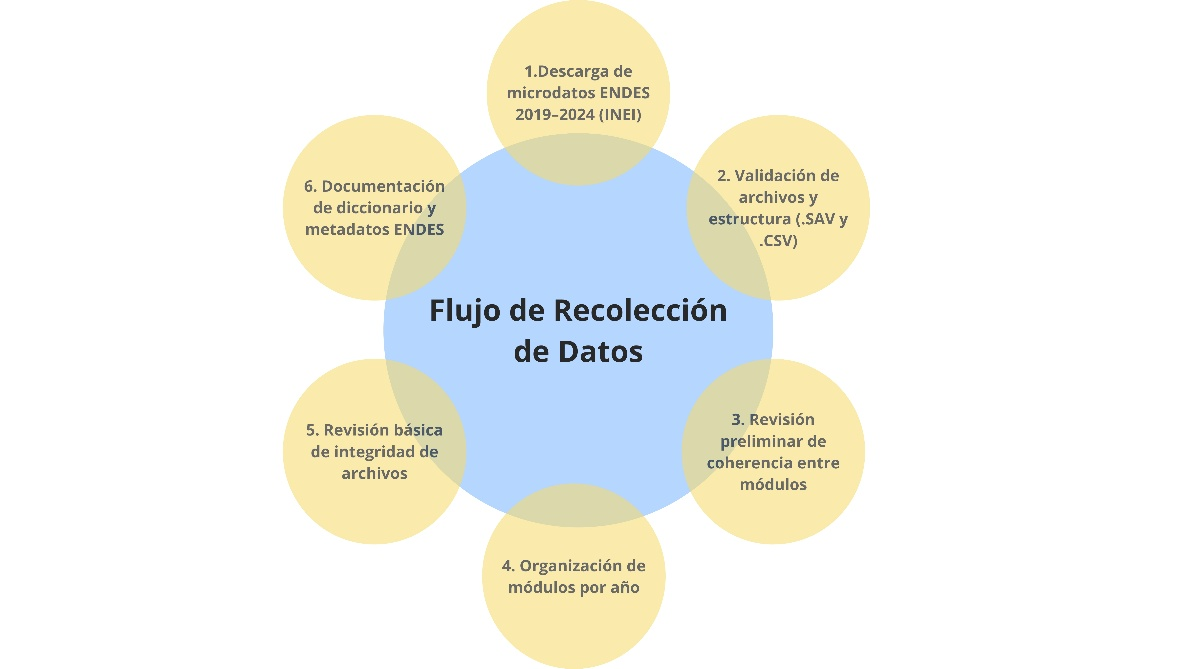
\includegraphics[width=5.39227in,height=3.03293in]{./media/image4.jpeg}
    
    \small Fig. 3. Flujo de Recolección de Datos -- ENDES 2019--2024
\end{center}

\hypertarget{tuxe9cnicas-estaduxedsticas-para-el-procesamiento-de-la-informaciuxf3n}{%
\subsection{2.4 Técnicas Estadísticas para el Procesamiento de la
Información}\label{tuxe9cnicas-estaduxedsticas-para-el-procesamiento-de-la-informaciuxf3n}}

Para el manejo de la información pequeña se usarán maneras de contar
pensadas para asegurar la pulcritud, firmeza y razón del cálculo que
anticipa cosas. El estudio que muestra lo obvio al principio tendrá
listas de cuántas veces pasan cosas, maneras de saber el medio y qué tan
separadas están las ideas, además de dibujos para mirar que dejen ver
formas del montón y posibles bichos raros en las tallas del cuerpo, de
la madre y de la plata {[}39{]}.

En el tiempo inicial de trabajo se usarán maneras propias acorde al tipo
de cosa que sea. Rellenar los huecos que faltan se hará con missForest,
un truco bien visto por su buen hacer en colecciones mezcladas de
números y etiquetas, y su forma de guardar lazos no rectos {[}31{]}. Las
cosas que cambian sin parar se pondrán a punto con la regla z-score, y
las que son de grupo se cambiarán con codificación de un solo indicio,
guardando la forma de base para que entren en las cajas de pensar
profundas. Por el desequilibrio propio de la poca comida en niños, se
usará SMOTE solo en la pila de práctica para no torcer las cosas y hacer
que el pensador note más las clases pequeñas {[}30{]}.

Para hacer que la muestra de información se vea mejor, se juntarán modos
de achicar y elegir partes, usando Kernel PCA y autoencoders de gráficos
profundos (dGAE), buenos para atrapar formas que no son rectas y moldes
de espacio escondidos {[}4, 10, 18{]}. De igual modo, se
usarán las formas MRMR y NRFS, escogidas porque saben cómo hacer que lo
importante crezca y lo repetido entre las cosas que dicen baje, lo cual
ayuda a que el aparato mezclado sea más fácil de entender y más rápido
de calcular {[}2, 32{]}.

En el punto de mirar las cosas, el patrón se probará con validación
cruzada de k-pliegues (k igual a diez), un modo bastante común para
calcular firmeza y notar escapes de datos (fuga de datos) mientras se
enseña {[}42{]}. Lo bueno de predecir se notará con precisión,
puntuación F1, sensatez, cualidad de no ser falso positivo y AUC-ROC,
dando más peso a las formas sólidas para situaciones donde las
categorías no están parejas {[}3{]}.

Finalmente, los resultados se presentarán mediante visualizaciones
generadas en Python, así como tableros interactivos en Power BI o
Streamlit, permitiendo una interpretación clara y accesible para los
actores técnicos y decisores del sector salud.

\hypertarget{aspectos-uxe9ticos-conducta-responsable-e-investigaciuxf3n---15-de-coincidencia}{%
\subsection{2.5 Aspectos Éticos (Conducta responsable e investigación -
15\% de
coincidencia)}\label{aspectos-uxe9ticos-conducta-responsable-e-investigaciuxf3n---15-de-coincidencia}}

\textbf{Cumplimiento ético institucional}

El estudio se desarrollará bajo los lineamientos éticos de la
Universidad Peruana Unión (UPeU) y de su Comité de Ética en
Investigación, garantizando integridad, transparencia y responsabilidad
en todas las etapas del proceso científico.

Aunque la investigación utiliza datos secundarios anonimizados y de
libre acceso, el proyecto será presentado para revisión institucional
conforme a los requisitos éticos establecidos por la UPeU {[}43{]}.

\textbf{Naturaleza de los datos}

El estudio empleará datos de la Encuesta Demográfica y de Salud Familiar
(ENDES) difundidos por el Instituto Nacional de Estadística e
Informática (INEI).

Estos microdatos:

\begin{itemize}
\item
  Son anonimizados,
\item
  Están disponibles en acceso abierto,
\item
  No requieren consentimiento informado ni contacto con personas.
\end{itemize}

Por ello, la investigación no implica intervención, ni riesgo para
individuos o comunidades {[}39{]}.

\textbf{Uso responsable de Inteligencia Artificial}

El uso de herramientas de Inteligencia Artificial se limitará a apoyo
académico en:

\begin{itemize}
\item
  Apoyo en redacción supervisada,
\item
  Comprensión metodológica,
\item
  Interpretación preliminar de resultados.
\end{itemize}

Todas las decisiones técnicas, científicas y analíticas serán
verificadas por el equipo investigador, siguiendo las directrices éticas
de la UNESCO y la OCDE para el uso responsable de IA.

\textbf{Verificación de similitud y originalidad}

El documento será sometido a herramientas oficiales de detección de
similitud, asegurando no superar el 15\% permitido por la UPeU.

Todas las citas, tablas, figuras y referencias serán correctamente
acreditadas bajo formato IEEE.

Se garantizará la originalidad del contenido, evitando plagio,
autoplagio o reutilización indebida de texto {[}43{]}.

\hypertarget{administraciuxf3n-del-proyecto}{%
\section{3. Administración del Proyecto}\label{administraciuxf3n-del-proyecto}}

\subsection{3.1 Cronograma de Actividades}\label{cronograma-de-actividades}

\begin{center}
    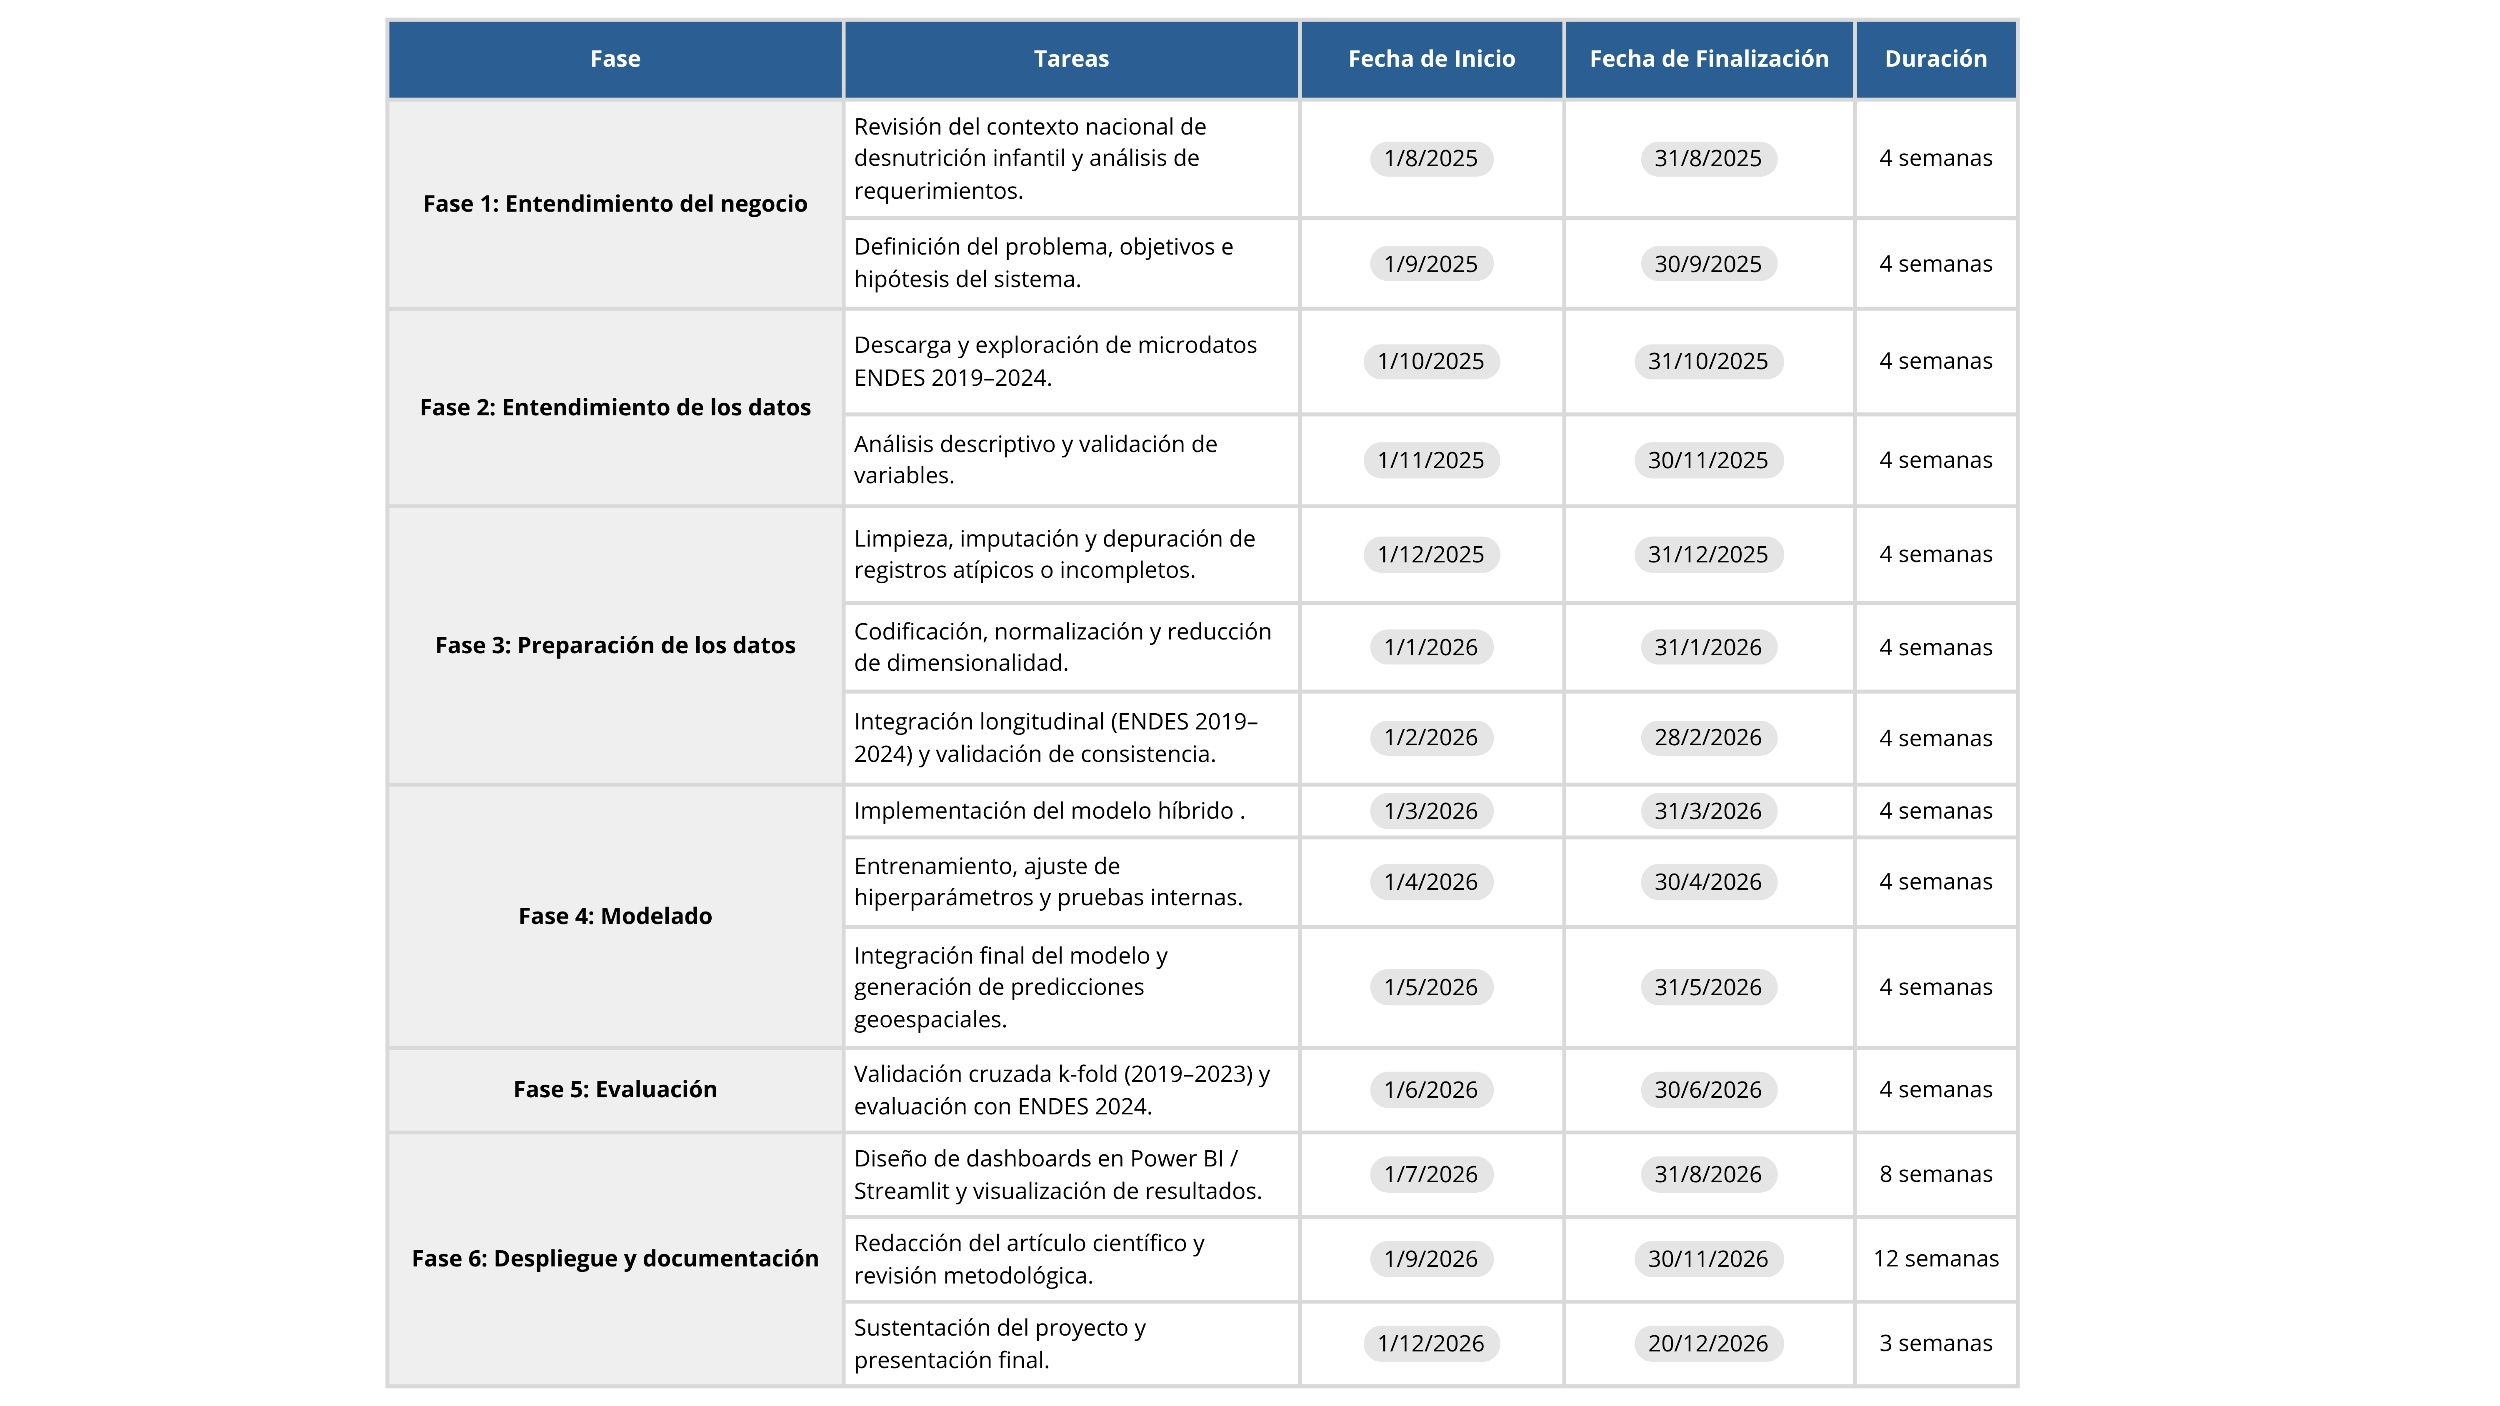
\includegraphics[width=0.9\linewidth]{./media/image5.jpeg}
    
    \small Tabla 1: Cronograma de Actividades Propuestas
\end{center}

\hypertarget{presupuesto-proyectado}{%
\subsection{3.2 Presupuesto Proyectado}\label{presupuesto-proyectado}}

\begin{longtable}[]{@{}
  >{\raggedright\arraybackslash}p{(\columnwidth - 4\tabcolsep) * \real{0.2404}}
  >{\raggedright\arraybackslash}p{(\columnwidth - 4\tabcolsep) * \real{0.6101}}
  >{\raggedright\arraybackslash}p{(\columnwidth - 4\tabcolsep) * \real{0.1495}}@{}}
\caption{Presupuesto Proyectado}\label{tab:presupuesto} \\
\toprule
\begin{minipage}[b]{\linewidth}\raggedright
\textbf{Concepto}
\end{minipage} & \begin{minipage}[b]{\linewidth}\raggedright
\textbf{Descripción}
\end{minipage} & \begin{minipage}[b]{\linewidth}\raggedright
\textbf{Costo (S/.)}
\end{minipage} \\
\midrule
\endhead
\textbf{Corrector o revisor de artículo (opcional)} & Servicio
especializado de revisión formal, ortotipográfica y de formato académico
(IEEE / Elsevier) previo a la publicación científica. & 350 \\
\textbf{Herramientas de software y visualización} & Uso de licencias
académicas y complementos técnicos para el análisis y representación de
datos (Power BI, RStudio, Netica, QGIS, Streamlit). & 500 \\
\textbf{Suscripción a entornos de cómputo e inteligencia artificial} &
Acceso a plataformas de entrenamiento y procesamiento en la nube (Google
Colab Pro, OpenAI API, HuggingFace) durante la fase de modelado. &
420 \\
\textbf{Almacenamiento en la nube} & Servicios de respaldo de datos y
modelos mediante Google Drive, GitHub o AWS durante el desarrollo del
sistema. & 240 \\
\textbf{Materiales y suministros} & Gastos asociados a impresiones,
encuadernado y elaboración de anexos físicos del informe final. & 150 \\
\textbf{Publicación del artículo científico (base)} & Tarifa de
publicación en revista indexada internacional (6 páginas base -- 625 EUR $\approx$ S/ 2,550). & 2,550 \\
\textbf{Página adicional del artículo} & Costo complementario por
extensión adicional del manuscrito (150 EUR $\approx$ S/ 610). & 610 \\
\textbf{Contingencia (10 \%)} & Margen destinado a imprevistos, ajustes
técnicos o costos administrativos menores. & 450 \\
\textbf{TOTAL ESTIMADO DEL PROYECTO} & & \textbf{5,270} \\
\bottomrule
\end{longtable}

\hypertarget{referencias-bibliogruxe1ficas}{%
\section{Referencias
Bibliográficas}\label{referencias-bibliogruxe1ficas}}

{[}1{]} World Health Organization, ``Global Report on Child Malnutrition
2024.'' Accessed: Oct. 09, 2025. {[}Online{]}. Available:
https://www.who.int/data/gho/data/themes/topics/joint-child-malnutrition-estimates-unicef-who-wb

{[}2{]} UNICEF, ``The State of the World's Children 2023: For Every
Child, Nutrition,'' New York, 2023. Accessed: Oct. 09, 2025.
{[}Online{]}. Available:
https://www.unicef.org/reports/state-worlds-children-2023\#SOWC

{[}3{]} United Nations, ``The Sustainable Development Goals Report.''

{[}4{]} C. G. Victora \emph{et al.}, ``Maternal and Child Undernutrition
2 Maternal and child undernutrition: consequences for adult health and
human capital,'' \emph{www.thelancet.com}, vol. 371, 2008, doi:
10.1016/S0140.

{[}5{]} L. C. Smith and L. Haddad, ``Reducing Child Undernutrition: Past
Drivers and Priorities for the Post-MDG Era,'' \emph{World Dev}, vol.
68, no. 1, pp. 180--204, Apr. 2015, doi: 10.1016/j.worlddev.2014.11.014.

{[}6{]} D. Kirk, E. Kok, M. Tufano, B. Tekinerdogan, E. J. M. Feskens,
and G. Camps, ``Machine Learning in Nutrition Research,'' \emph{Advances
in Nutrition}, vol. 13, no. 6, pp. 2573--2589, Nov. 2022, doi:
10.1093/advances/nmac103.

{[}7{]} A. Hendy \emph{et al.}, ``Unlocking insights: Using machine
learning to identify wasting and risk factors in Egyptian children under
5,'' \emph{Nutrition}, vol. 131, Mar. 2025, doi:
10.1016/j.nut.2024.112631.

{[}8{]} J. Khan, A. Alam, and Y. Lee, ``Intelligent Hybrid Feature
Selection for Textual Sentiment Classification,'' \emph{IEEE Access},
vol. 9, pp. 140590--140608, 2021, doi: 10.1109/ACCESS.2021.3118982.

{[}9{]} W. Hadikurniawati, K. D. Hartomo, I. Sembiring, and C. Arthur,
``A Dual-Fusion Hybrid Model with Attention for Stunting Prediction
among Children under Five Years,'' \emph{Journal of Applied Data
Sciences}, vol. 6, no. 3, pp. 1985--1998, 2025, doi:
10.47738/jads.v63.831.

{[}10{]} F. G. Habtewold and B. G. Arero, ``Modeling and mapping
under-nutrition among under-five children in Ethiopia: a Bayesian
spatial analysis,'' \emph{Front Public Health}, vol. 13, 2025, doi:
10.3389/fpubh.2025.1553908.

{[}11{]} O. A. Egbon, A. M. Belachew, and M. A. Bogoni, ``Risk factors
of concurrent malnutrition among children in Ethiopia: a bivariate
spatial modeling approach,'' \emph{All Life}, vol. 15, no. 1, pp.
512--536, 2022, doi: 10.1080/26895293.2022.2067251.

{[}12{]} E. Malinowski, ``Challenges for promoting the decision-making
processes based on spatial data analysis,'' \emph{Smart Innovation,
Systems and Technologies}, vol. 20, pp. 393--402, 2013, doi:
10.1007/978-3-642-35452-6\_40.

{[}13{]} W. R. Mgomezulu, P. Thangata, B. Mkandawire, and N. Amoah,
``Advancing predictive analytics in child malnutrition: Machine,
ensemble and deep learning models with balanced class distribution for
early detection of stunting and wasting,'' \emph{Human Nutrition and
Metabolism}, vol. 42, Dec. 2025, doi: 10.1016/j.hnm.2025.200340.

{[}14{]} K. Luijken \emph{et al.}, ``Changing predictor measurement
procedures affected the performance of prediction models in clinical
examples,'' \emph{J Clin Epidemiol}, vol. 119, pp. 7--18, Mar. 2020,
doi: 10.1016/j.jclinepi.2019.11.001.

{[}15{]} Instituto Nacional de Estadística e Informática (INEI),
``Desnutrición crónica infantil afectó al 11,5 \% de niñas y niños
menores de cinco años en 2023.'' Accessed: Nov. 11, 2025. {[}Online{]}.
Available:
https://m.inei.gob.pe/prensa/noticias/el-431-de-la-poblacion-de-6-a-35-meses-de-edad-sufrio-de-anemia-en-el-ano-2023-15077/

{[}16{]} Ministerio de Salud (MINSA), ``MINSA articula trabajo
multisectorial para mejorar la seguridad alimentaria y la
malnutrición,'' Gobierno del Perú -- Ministerio de Salud. Accessed: Nov.
11, 2025. {[}Online{]}. Available:
https://www.gob.pe/institucion/minsa/noticias/1063004-minsa-articula-trabajo-multisectorial-para-mejorar-la-seguridad-alimentaria-y-la-malnutricion

{[}17{]} T. P. Theodore Armand, K. A. Nfor, J. I. Kim, and H. C. Kim,
``Applications of Artificial Intelligence, Machine Learning, and Deep
Learning in Nutrition: A Systematic Review,'' Apr. 06, 2024. doi:
10.3390/nu16071073.

{[}18{]} M. M. Alam, A. I. Khan, A. Zafar, M. Sohail, M. T. Ahmad, and
R. Azim, ``Advancing Nutritional Status Classification With Hybrid
Artificial Intelligence: A Novel Methodological Approach,'' \emph{Brain
Behav}, vol. 15, no. 5, May 2025, doi: 10.1002/brb3.70548.

{[}19{]} B. Rao, M. Rashid, M. G. Hasan, and G. Thunga, ``Machine
Learning in Predicting Child Malnutrition: A Meta-Analysis of
Demographic and Health Surveys Data,'' Mar. 01, 2025,
\emph{Multidisciplinary Digital Publishing Institute (MDPI)}. doi:
10.3390/ijerph22030449.

{[}20{]} N. Hasdyna, R. K. Dinata, Rahmi, and T. I. Fajri, ``Hybrid
Machine Learning for Stunting Prevalence: A Novel Comprehensive Approach
to Its Classification, Prediction, and Clustering Optimization in Aceh,
Indonesia,'' \emph{Informatics}, vol. 11, no. 4, Dec. 2024, doi:
10.3390/informatics11040089.

{[}21{]} R. Qasrawi \emph{et al.}, ``Machine Learning Approach for
Predicting the Impact of Food Insecurity on Nutrient Consumption and
Malnutrition in Children Aged 6 Months to 5 Years,'' \emph{Children},
vol. 11, no. 7, Jul. 2024, doi: 10.3390/children11070810.

{[}22{]} G. Nduwayezu \emph{et al.}, ``Spatial Machine Learning for
Exploring the Variability in Low Height-For-Age From Socioeconomic,
Agroecological, and Climate Features in the Northern Province of
Rwanda,'' \emph{Geohealth}, vol. 8, no. 9, Sep. 2024, doi:
10.1029/2024GH001027.

{[}23{]} D. B. Rahut, R. Mishra, and S. Bera, ``Geospatial and
environmental determinants of stunting, wasting, and underweight:
Empirical evidence from rural South and Southeast Asia,''
\emph{Nutrition}, vol. 120, Apr. 2024, doi: 10.1016/j.nut.2023.112346.

{[}24{]} L. A. Jokhu and A. Syauqy, ``Determinants of concurrent wasting
and stunting among children 6 to 23 mo in Indonesia,'' \emph{Nutrition},
vol. 122, Jun. 2024, doi: 10.1016/j.nut.2024.112390.

{[}25{]} P. Jasper, W. C. Jochem, E. Lambert-Porter, U. Naeem, and C. E.
Utazi, ``Mapping the prevalence of severe acute malnutrition in Papua,
Indonesia by using geostatistical models,'' \emph{BMC Nutr}, vol. 8, no.
1, Dec. 2022, doi: 10.1186/s40795-022-00504-z.

{[}26{]} D. Backer and T. Billing, ``Validating Famine Early Warning
Systems Network projections of food security in Africa, 2009--2020,''
\emph{Glob Food Sec}, vol. 29, Jun. 2021, doi:
10.1016/j.gfs.2021.100510.

{[}27{]} G. A. Tadesse \emph{et al.}, ``Forecasting acute childhood
malnutrition in Kenya using machine learning and diverse sets of
indicators,'' \emph{PLoS One}, vol. 20, no. 5 May, May 2025, doi:
10.1371/journal.pone.0322959.

{[}28{]} B. Baffour, J. M. K. Aheto, S. Das, P. Godwin, and A.
Richardson, ``Geostatistical modelling of child undernutrition in
developing countries using remote-sensed data: evidence from Bangladesh
and Ghana demographic and health surveys,'' \emph{Sci Rep}, vol. 13, no.
1, Dec. 2023, doi: 10.1038/s41598-023-48980-y.

{[}29{]} W. Hadikurniawati, K. D. Hartomo, I. Sembiring, and C. Arthur,
``A Dual-Fusion Hybrid Model with Attention for Stunting Prediction
among Children under Five Years,'' \emph{Journal of Applied Data
Sciences}, vol. 6, no. 3, pp. 1985--1998, 2025, doi:
10.47738/jads.v63.831.

{[}30{]} H. A. Santoso, N. S. Dewi, S. C. Haw, A. D. Pambudi, and S. A.
Wulandari, ``Enhancing nutritional status prediction through
attention-based deep learning and explainable AI,'' \emph{Intell Based
Med}, vol. 11, Jan. 2025, doi: 10.1016/j.ibmed.2025.100255.

{[}31{]} S. Constenla-Villoslada, Y. Liu, L. McBride, C. Ouma, N.
Mutanda, and C. B. Barrett, ``High-frequency monitoring enables machine
learning--based forecasting of acute child malnutrition for early
warning,'' \emph{Proc Natl Acad Sci U S A}, vol. 122, no. 23, Jun. 2025,
doi: 10.1073/pnas.2416161122.

{[}32{]} J. Castro-Bedriñana, D. Chirinos-Peinado, and G. De La
Cruz-Calderón, ``Predictive model of stunting in the Central Andean
region of Peru based on socioeconomic and agri-food determinants,''
\emph{Public Health in Practice}, vol. 2, Nov. 2021, doi:
10.1016/j.puhip.2021.100112.

{[}33{]} R. Wirth and J. Hipp, ``CRISP-DM: Towards a Standard Process
Model for Data Mining.''

{[}34{]} T. D. Le, R. Noumeir, J. Rambaud, G. Sans, and P. Jouvet,
``Adaptation of Autoencoder for Sparsity Reduction From Clinical Notes
Representation Learning,'' \emph{IEEE J Transl Eng Health Med}, vol. 11,
pp. 469--478, 2023, doi: 10.1109/JTEHM.2023.3241635.

{[}35{]} N. V Chawla, K. W. Bowyer, L. O. Hall, and W. P. Kegelmeyer,
``SMOTE: Synthetic Minority Over-sampling Technique,'' 2002.

{[}36{]} Z. Chen, Z. Lao, Y. Lu, W. Zhang, A. Edwards, and K. Zhang,
``Decoding ancestry-specific genetic risk: interpretable deep feature
selection reveals prostate cancer SNP disparities in diverse
populations,'' \emph{BioData Min}, vol. 18, no. 1, Dec. 2025, doi:
10.1186/s13040-025-00470-9.

{[}37{]} R. Kohavi, ``A Study of Cross-Validation and Bootstrap for
Accuracy Estimation and Model Selection.'' {[}Online{]}. Available:
http//roboticsStanfordedu/"ronnyk

{[}38{]} FAO, UNICEF, and WHO, \emph{The State of Food Security and
Nutrition in the World 2023}. FAO; IFAD; UNICEF; WFP; WHO;, 2023. doi:
10.4060/cc3017en.

{[}39{]} Instituto Nacional de Estadística e Informática (INEI), ``Base
de Microdatos ENDES,'' INEI. Accessed: Nov. 11, 2025. {[}Online{]}.
Available: https://proyectos.inei.gob.pe/microdatos/

{[}40{]} World Health Organization (WHO), ``Length/height-for-age,
weight-for-age, weight-for-length, weight-for-height and body mass
index-for-age Methods and development.''

{[}41{]} X. Wu, L. Wang, M. Ge, J. Jiang, Y. Cai, and B. Yang,
``Adaptive biases-incorporated latent factorization of tensors for
predicting missing data in water quality monitoring networks,''
\emph{Front Phys}, vol. 13, 2025, doi: 10.3389/fphy.2025.1587012.

{[}42{]} M. Becker, J. Lippel, A. Stuhlsatz, and T. Zielke, ``Robust
dimensionality reduction for data visualization with deep neural
networks,'' \emph{Graph Models}, vol. 108, Mar. 2020, doi:
10.1016/j.gmod.2020.101060.

{[}43{]} Universidad Peruana Unión (UpeU), ``Código de Ética en
Investigación Científica.'' Accessed: Nov. 11, 2025. {[}Online{]}.
Available: https://investigacion.upeu.edu.pe/comite-de-etica/

~

\hypertarget{anexo-a}{%
\section{Anexo A}\label{anexo-a}}

\hypertarget{instrumentos-de-recolecciuxf3n-de-datos}{%
\subsection{Instrumentos de Recolección de
Datos}\label{instrumentos-de-recolecciuxf3n-de-datos}}

En caso de estudios con instrumentos, se debe incluir una copia en
blanco del instrumento completo, incluyendo su consentimiento informado.

\hypertarget{anexo-b}{%
\section{Anexo B}\label{anexo-b}}

\hypertarget{matriz-de-operacionalizaciuxf3n-de-variables}{%
\subsection{Matriz de operacionalización de
variables}\label{matriz-de-operacionalizaciuxf3n-de-variables}}

Solo para estudios con variable(s) social(es).

\hypertarget{anexo-c}{%
\section{Anexo C}\label{anexo-c}}

\hypertarget{imuxe1genes-planos-figuras-tablas-u-otros}{%
\subsection{Imágenes, planos, figuras, tablas u
otros}\label{imuxe1genes-planos-figuras-tablas-u-otros}}

Opcionales, según la metodología aplicada.

\end{document}
